\documentclass[12pt]{article}
\usepackage[top=2cm]{geometry}
\usepackage{amsmath}
\usepackage{amsthm}
\usepackage{amsfonts}
\usepackage{parskip}
\usepackage{graphicx}
\graphicspath{ {images/} }

\title{\textbf{MPLS and VPNs}}
\author{}
\date{}

\begin{document}
\maketitle

\section*{MPLS}

The logical connection between two routers is based on a lightpath (optical network).
The connection is provided by an ISP (Layer 3 network).

The most crucial function of an IP network is routing, finding a path from one client to another.
Routing tables are filled with shortest path algorithms on graphs (Dijkstra).

Sometimes, IP routing is not the most efficient choice. 

\begin{figure}[ht]
    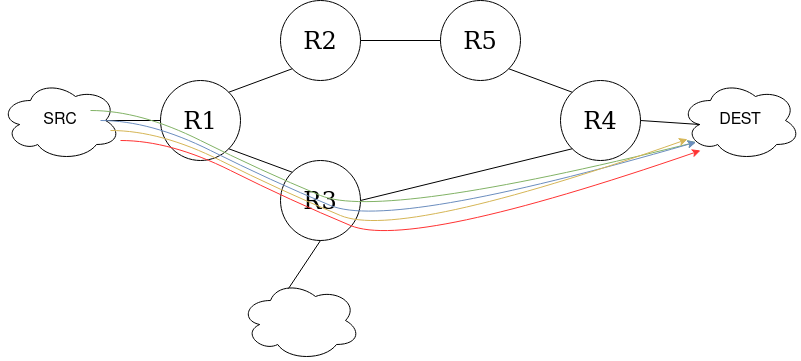
\includegraphics[scale = 0.4]{Example1.png}
    \centering
    \caption[short]{Traffic through \(R_1 \rightarrow R_3 \rightarrow R_4\)}
\end{figure}

Multiple clients may send traffic through a path because it's the shortest,but this leads to overloading the path.

This is where "traffic engineering" comes into play. It's about distributing data traffic more efficiently across the network.

Traffic engineering is a function that ISPs must provide. VPNs are private paths between two hosts on a public network. It's created to establish a private network between two hosts not physically connected on the same network. The packets sent have the recipient's private IP, but the packet is encapsulated and sent through MPLS.

\newpage
In MPLS, the routing table associates the paths that packets should take.

\begin{figure}[ht]
    \includegraphics[scale = 0.3]{connectionOriented.png}
    \centering
\end{figure}

In the IN column, the first number corresponds to the incoming port where the packet is received, and the second number is the corresponding label for the packet. In the OUT column, the corresponding outgoing port and label.

The label is a part of the header with a number.

This type of connection simulates a tunnel between two hosts on the public network.

\begin{figure}[ht]
    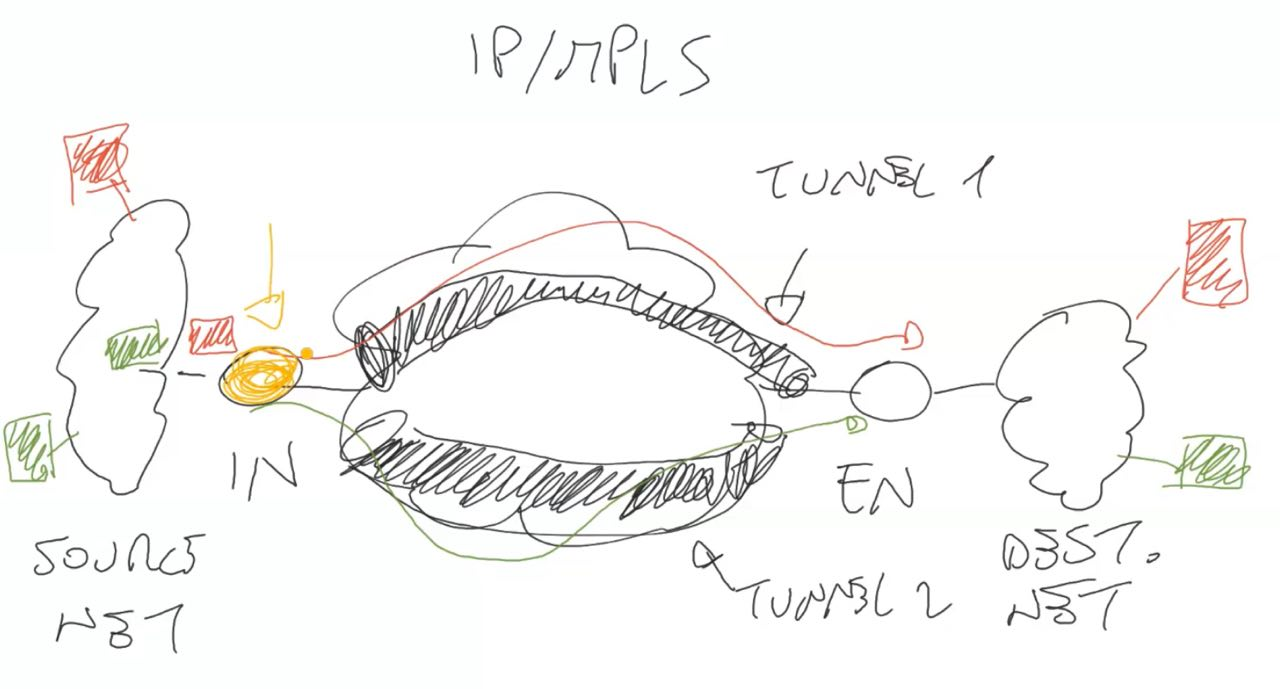
\includegraphics[scale = 0.3]{Example2.jpeg}
    \centering
\end{figure}
When two packets need to be sent into the network via two tunnels, a routing function called a "classifier" decides where to send the packets.

\newpage
Classification is done based on the following criteria:
\begin{itemize}
    \item src IP
    \item dst IP
    \item protocol
    \item src port
    \item dst port
\end{itemize}
    
The next step is to remove MPLS from the OSI model stack to allow it to be replaced by IPv6.

MPLS labels are carried in an MPLS header. They are inserted between Layer 2 and Layer 3. MPLS supports multilevel encapsulation, where you can add an MPLS label stack on top of an IP packet, with the lowest label corresponding to the last header.

The Ingress LER of an MPLS domain analyzes the IP header of the packet, classifies the packet, adds the MPLS label, and forwards it to the next hop LSR. In the MPLS domain, the packet is forwarded along the LSP according to the labels. The Egress LER removes the label, and the packet is forwarded based on the IP destination address.

Three basic actions:
    PUSH operation: Add the MPLS label.
    POP operation: Remove the MPLS label.
    SWAP operation: Change the label (in an intermediate node).

The SWAP operation is performed by a Label Switched Router.

It is possible to decide whether to use MPLS or the IP protocol. To use the latter, insert the number 0000 in the label designated for MPLS, and the packet will be forwarded through the IP protocol.

3 pros of MPLS are 
\begin{itemize}
    \item VPNs
    \item Traffic engineering
    \item Fast restoration
\end{itemize}


\newpage
\section*{VPN, Traffic Engineering and Fast Re-Route}

\subsection*{VPNs}
\begin{figure}[ht]
    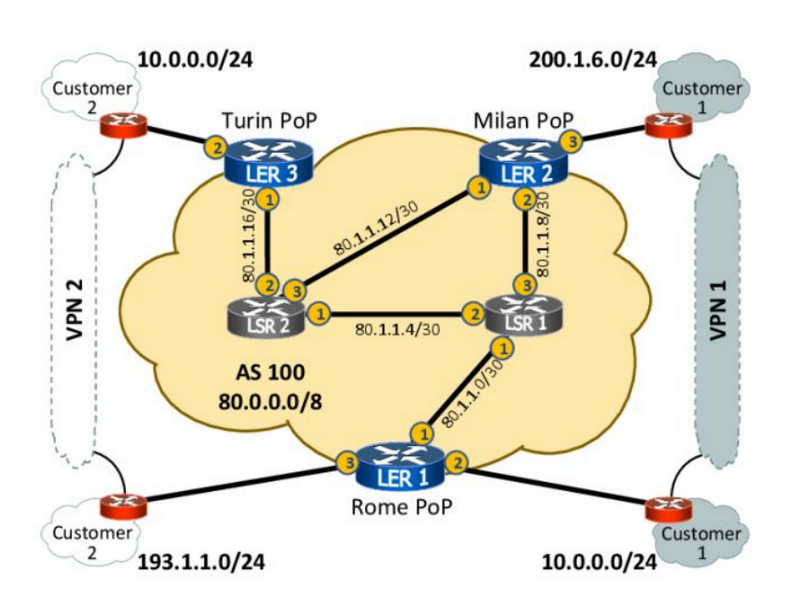
\includegraphics[scale = 0.4]{Example3.png}
    \centering
\end{figure}

In the example in the figure, there are two companies, both with hosts located far apart. Communication between them needs to be private, as if they were communicating on the same network. One way to achieve this is through a VPN.

Taking the example in the figure, 193.1.1.0/24 is in Rome, while 10.0.0.0/24 
is in Turin. When using a VPN, the source (src) and destination (dest) IP addresses are both private.

Please insert the figure at minute 19.

It's possible to create a VPN in an MPLS network in three steps.

\subsubsection*{Move 1: Any-to-any IP connectivity among PEs}

Assigning a specific identifier, a well-defined IP address, 
to each device in the network is important for easy identification. 
Another reason for this practice is that if the physical network card address were assigned, it might not always be reachable, as the network card could be down for various reasons. 
By using IP addresses, you ensure constant reachability.

\newpage
\subsubsection*{Move 2: Use BGP to distribute customer prefixes. }

Through a BGP message, an autonomous system sends information about 
the devices reachable through it to other routers. 
BGP (Border Gateway Protocol) is used to exchange routing and reachability information among different autonomous systems (ASes) on the Internet. It plays a crucial role in determining the best path for data to travel across the internet, helping routers 
make informed decisions about how to forward data packets.

\begin{figure}[ht]
    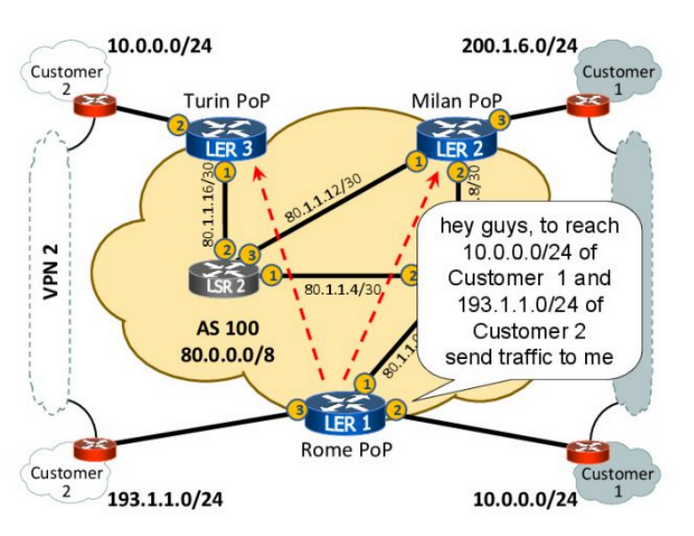
\includegraphics[scale = 0.4]{Example4.png}
    \centering
\end{figure}

One problem with BGP is that it communicates a series of private IP 
addresses, which means that other routers may not know how to 
reach those private IP addresses. 
To address this issue, Multi-Protocol BGP (MP-BGP) is used. MP-BGP 
communicates, along with the private IP addresses, information about which customer they belong to. This type of identification is called L3VPN (Layer 3 Virtual Private Network). L3VPNs are a way to provide private network services over a shared network infrastructure, and MP-BGP is an essential protocol for establishing and managing these virtual private networks.
\newpage
\subsubsection*{Move 3: Use MPLS encapsulation among PEs}

\begin{figure}[ht]
    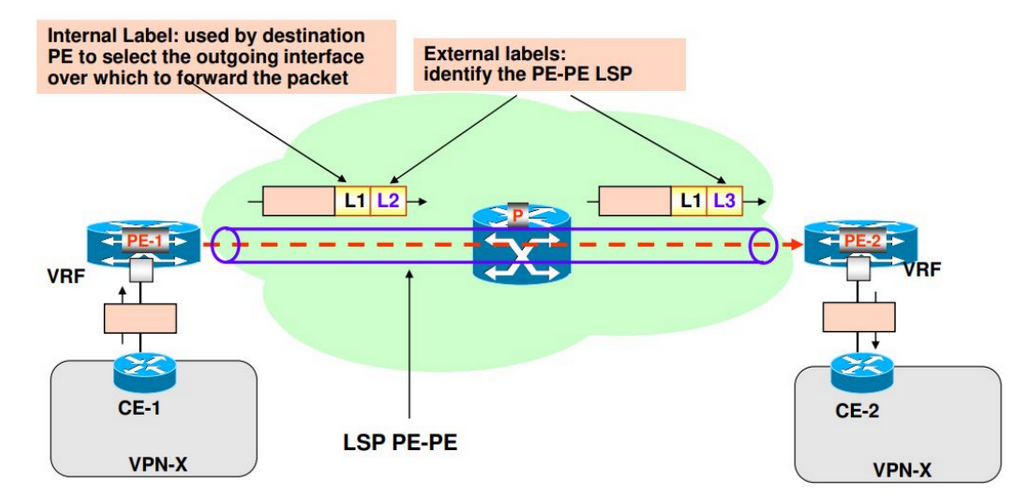
\includegraphics[scale = 0.4]{Example5.png}
    \centering
\end{figure}

To create a private network within a public network, you need to establish a tunnel, and MPLS (Multi-Protocol Label Switching) is commonly used for this purpose. In VPNs (Virtual Private Networks), an additional label is needed beyond the forwarding label.

MPLS is a technology that enhances the efficiency and security of data transmission in networks. It does so by assigning a label to each data packet, allowing routers to make forwarding decisions based on these labels. In the context of VPNs, MPLS is used to create a tunnel for private network traffic within a shared, public network.

The additional label in VPNs is often used to indicate to which specific customer or virtual private network the data packet belongs. This label is crucial for routers to correctly route the data within the VPN, ensuring that it reaches the intended destination securely and privately.

Esempio al minuto 40. 

In this example, if there were no second label, the router in Rome would receive a packet destined for the private network 10.0.0.0/2410.0.0.0/24. 
However, there are two instances of this network, and without the second label, the router would not know which customer to forward the packet to. 
The second label is essential for this purpose, as it helps the router determine which customer's private network the packet belongs to. This additional layer of labeling in MPLS networks, known as the VPN label, 
is what enables routers to correctly route the packet within the multi-customer network and ensure that it reaches the appropriate destination.
\newpage
\subsubsection*{Routing tables}

\begin{figure}[ht]
    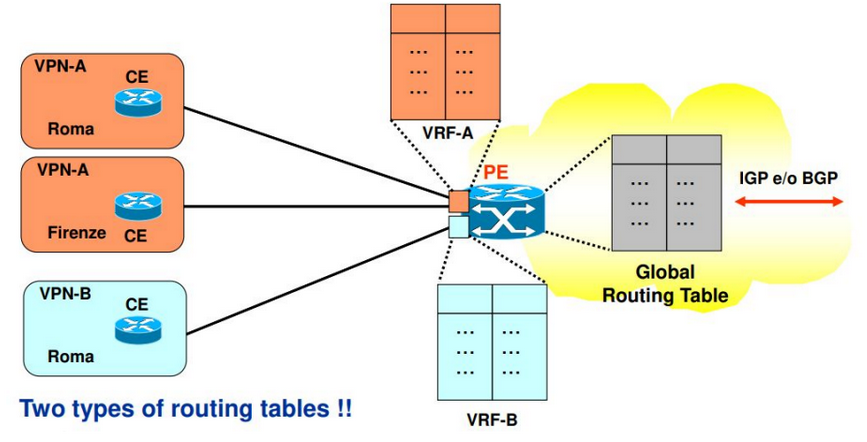
\includegraphics[scale = 0.4]{Example7.png}
    \centering
\end{figure}

Exactly, when a router receives a packet from two different customers with identical private IP addresses, it needs to maintain separate routing tables or contexts for each customer. This separation is necessary to distinguish between the two customers and to determine the correct path for forwarding the packet. Once the router has identified which customer the packet belongs to, it can then send it to the appropriate destination with certainty. This separation of routing information ensures that each customer's traffic is kept private and is routed correctly within the multi-customer network, which is a key aspect of MPLS-based VPNs.

\subsection*{Traffic Engineering}

An external entity chooses the path and then the routers are configured accordingly. 

The routers autonomously choose the path that follow some Quality o Services constraint. 

The path is chosen for each new LSP to be setup (“on-line”).

Global optimization (“off-line”) on all paths in the network.

\newpage
\subsection*{Fast-Reroute}

\begin{figure}[ht]
    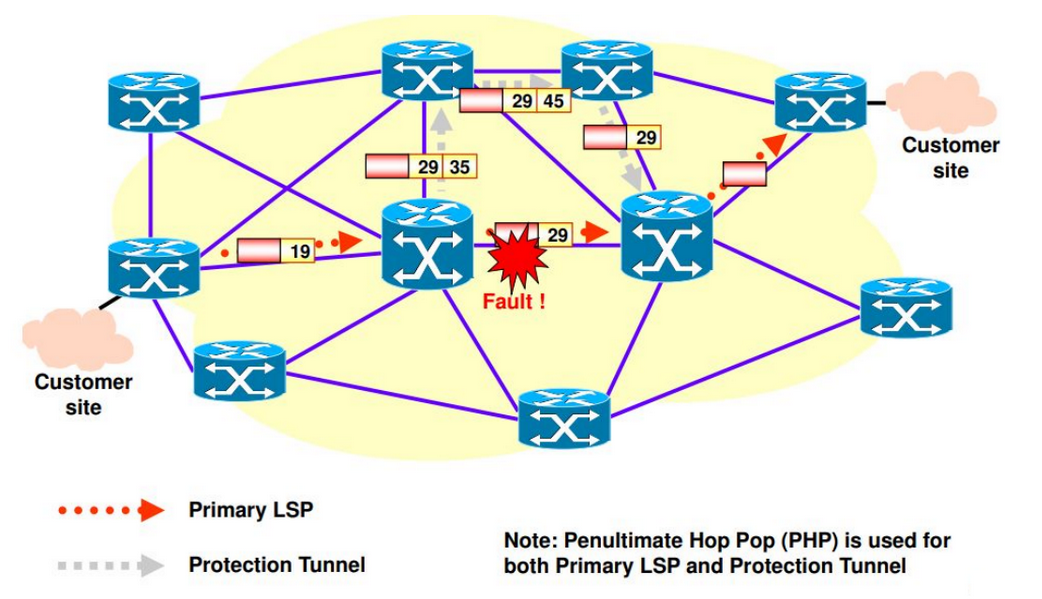
\includegraphics[scale = 0.4]{Example8.png}
    \caption{Link protection}
    \centering
\end{figure}

\begin{figure}[ht]
    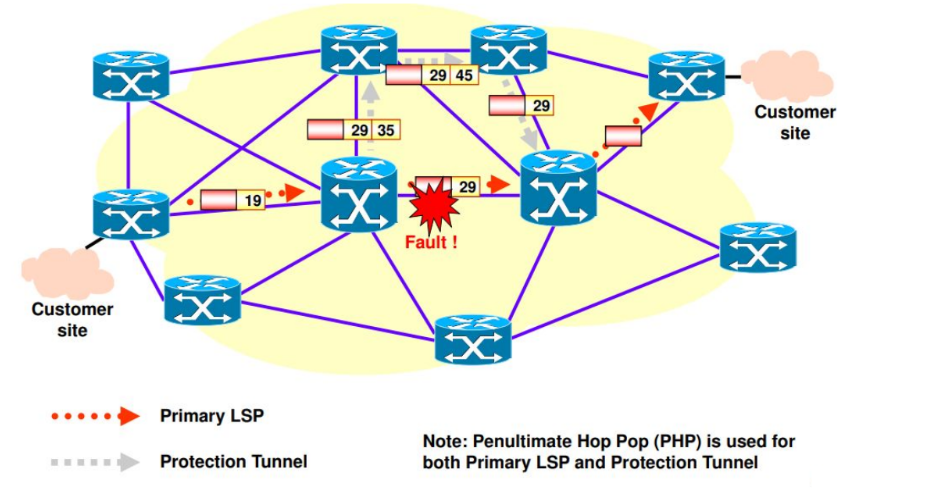
\includegraphics[scale = 0.40]{Example9.png}
    \caption{Link protection}
    \centering
\end{figure}

\end{document}